\part{Preliminaries}




\chapter[Introduction]{Introduction}
\label{sec:introduction}


\section{What is pbd?}

The ``Programming with Big Data in R'' project~\citep{pbdR2012} (pbd or pbdR for short) is a project that aims to elevate the statistical programming language \proglang{R}~\citep{Rcore} to leadership-class computing platforms.  
\begin{figure}[t]
 \centering
 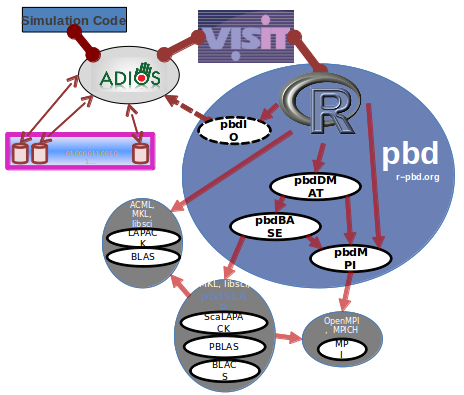
\includegraphics{pbdDEMO-include/pics/pbd}
 \caption{pbdR Packages and Their Relationships with Scalable Libraries}
 \label{fig:pbdrpackages}
\end{figure}
Figure~\ref{fig:pbdrpackages} shows the current state of pbdR packages and how they utilize proven, high-performance, scalable libraries and visualization tools.  More explicitly, the current pbdR packages are:

\begin{itemize}
 \item \pkg{pbdMPI} --- an efficient interface to MPI with a focus on Single Program/Multiple Data (SPMD) parallel programming style.
 \item \pkg{pbdSLAP} --- bundles scalable dense linear algebra libraries in double precision for \pkg{R}, based on ScaLAPACK version 2.0.2~\citep{slug}..
 \item \pkg{pbdNCDF4} --- Interface to Parallel Unidata NetCDF4 format data files~\citep{netcdf}.
 \item \pkg{pbdBASE} --- base distributed classes and methods for the pbdR Project.
 \item \pkg{pbdDMAT} --- distributed matrix computational methods, with a focus on linear algebra.
 \item \pkg{pbdDEMO} --- set of package demonstrations and examples, and this unifying vignette.
\end{itemize}

In this vignette, we offer many examples using the above pbdR packages.  Many of the examples are high-level
applications and may be commonly found in basic Statistics.  The purpose is to show how to reuse the pre-existing functions and utilities of pbdR to create minor extensions which can quickly solve problems in an efficient way.  The reader is encouraged to reuse and repurpose these functions.

The \pkg{pbdDEMO} package consists of two main parts.  The first is a collection of roughly 15 package demos.  These offer example uses of the various pbdR packages.  The second is this vignette, which attempts to offer detailed explanations for the demos, as well as sometimes providing some mathematical or statistical insight.  A list of all of the package demos can be found in Section~\ref{sec:demolist}.



\section{Why Parallelism?  Why pbdR?}

It is common, in a document such as this, to justify the need for parallelism.  Generally this process goes:

\begin{quote}
\emph{
Blah blah blah Moore's Law, blah blah Big Data, blah blah blah Concurrency.
}
\end{quote}

How about this?  Parallelism is cool.  Any boring nerd can use one computer, but using 10,000 at once is another story.  We don't call them \emph{\textbf{supercomputers}} for nothing.

But unfortunately, lots of people who would otherwise be thrilled to do all kinds of cool stuff with massive behemoths of computation~--- computers with names like \textbf{KRAKEN} and \textbf{TITAN}~--- are burdened by an unfortunate reality:  it's really, really hard.  Enter pbdR.  Through our project, we put a shiny new set of clothes on high-powered compiled code, making massive-scale computation accessible to a wider audience of data scientists than ever before.  Analytics in supercomputing shouldn't just be for the elites.



\section[Installation]{Installation}
\label{sec:installation}

One can download \pkg{pbdDEMO} from CRAN at
\url{http://cran.r-project.org}, and
the intallation can be done with the following commands
\begin{lstlisting}
tar zxvf pbdDEMO_0.1-0.tar.gz
R CMD INSTALL pbdDEMO
\end{lstlisting}
Since \pkg{pbdEMO} depends on other pbdR packages, please read the corresponding vignettes if installation of any of them is unsuccessful.


\section{List of Demos}
\label{sec:demolist}

A full list of demos contained in the \pkg{pbdDEMO} package is provided below.

\begin{lstlisting}[title=Shell Script]
### (Use Rscript.exe for windows system)


		      # --------------------- #
		      # II Direct MPI Methods #
		      # --------------------- #

### Chapter 5
# Monte carlo simulation
mpiexec -np 4 Rscript -e "demo(monte_carlo, package='pbdDMAT', ask=F, echo=F)"
# Sample mean and variance
mpiexec -np 4 Rscript -e "demo(sample_stat, package='pbdDMAT', ask=F, echo=F)"
# Binning
mpiexec -np 4 Rscript -e "demo(binning, package='pbdDMAT', ask=F, echo=F)"
# Quantile
mpiexec -np 4 Rscript -e "demo(quantile, package='pbdDMAT', ask=F, echo=F)"
# OLS
mpiexec -np 4 Rscript -e "demo(ols, package='pbdDMAT', ask=F, echo=F)"


		  # ----------------------------- #
		  # III Reading and Managing Data #
		  # ----------------------------- #

### Chapter 6
# Random matrix generation
mpiexec -np 4 Rscript -e "demo(randmat_global, package='pbdDMAT', ask=F, echo=F)"
mpiexec -np 4 Rscript -e "demo(randmat_local, package='pbdDMAT', ask=F, echo=F)"

### Chapter 7
# Reading csv
mpiexec -np 4 Rscript -e "demo(read_csv, package='pbdDMAT', ask=F, echo=F)"
# Reading sql
mpiexec -np 4 Rscript -e "demo(read_sql, package='pbdDMAT', ask=F, echo=F)"
# Reading netcdf4
mpiexec -np 4 Rscript -e "demo(read_ncdf, package='pbdDMAT', ask=F, echo=F)"

### Chapter 8
# Loand/unload balance
mpiexec -np 4 Rscript -e "demo(balance, package='pbdDMAT', ask=F, echo=F)"
# SPMD to DMAT
mpiexec -np 4 Rscript -e "demo(spmd_dmat, package='pbdDMAT', ask=F, echo=F)"
# Distributed matrix redistributions
mpiexec -np 4 Rscript -e "demo(reblock, package='pbdDMAT', ask=F, echo=F)"

		  # ----------------------------- #
		  # IV Distributed Matrix Methods #
		  # ----------------------------- #

### Chapter 9
# Verify solveing Ax=b at scale
mpiexec -np 4 Rscript -e "demo(verify, package='pbdDMAT', ask=F, echo=F)"
# PCA compression
mpiexec -np 4 Rscript -e "demo(pca, package='pbdDMAT', ask=F, echo=F)"
# OLS and predictions
mpiexec -np 4 Rscript -e "demo(ols_dmat, package='pbdDMAT', ask=F, echo=F)"
\end{lstlisting}